\section{Problem 3}
\label{part3}
\begin{verbatim}
Now rank the same 10 URIs from question #2, but this time 
by their PageRank.  Use any of the free PR estimaters on the web,
such as:

http://www.prchecker.info/check_page_rank.php
http://www.seocentro.com/tools/search-engines/pagerank.html
http://www.checkpagerank.net/

If you use these tools, you'll have to do so by hand (they have
anti-bot captchas), but there is only 10.  Normalize the values
they give you to be from 0 to 1.0.  Use the same tool on all 10
(again, consistency is more important than accuracy).

Create a table similar to Table 1:

Table 2.  10 hits for the term "shadow", ranked by PageRank.

PageRank	URI
--------	---
0.9		http://bar.com/
0.5		http://foo.com/

Briefly compare and contrast the rankings produced in questions 2
and 3.

\end{verbatim}
\subsection{Solution}
\begin{enumerate}

\item For this question I need to get the Page rank for each of the 10 URIs.
\item This can be found out by using one of the 3 links provided in the question.  
\item I used 2nd link as it did not ask captcha to enter each time I check for a rank. This just reduced my work a little bit.
\item I manually copied each URI and pasted it in the PR estimator website and it gave me the rank.
\item First when I tried to get the rank from my URIs all my 10 URIs gave n/a output.
\item Later I read the comment in the google groups and found that it can use top-level URIs rather than my entire URI.
\item This is because deep links into a site does not have PR.
\item So I took top level of each URI and got the Page rank for each one of them. This can be seen in Figure 9.
\item Now each Page rank is normalized as asked in the question. 
\item The list of Page ranks arranged in ascending order and the URIs are shown in Figure 10.
\item In the question I was asked to compare Page rank and TFIDF, so both of them are shown in a single table which can be seen in Figure 11.
\item When we compare the rankings based on TFIDF and page rank there is not relation between them.Page rank considers back link structures,so it gives the rank of the document with respect to other documents in the web,but TFIDF gives rank to the documents based on the level of similarity to the term.So If a document has high TFIDF value then it ranks it high even though if it is unpopular. 
\newpage
\end{enumerate}
\subsection{Results}

\subsubsection{Sample Rank for one URI}
\begin{figure}[ht]    
    \begin{center}
        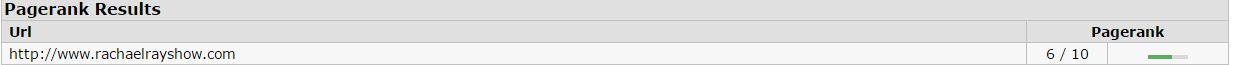
\includegraphics[scale=0.5]{sample_rank.png}
        \caption{Sample Rank for one URI}
        \label{Sample Rank for one URI}
    \end{center}
\end{figure}

\subsubsection{Page rank along with 10 URIs}
\begin{figure}[ht]    
    \begin{center}
        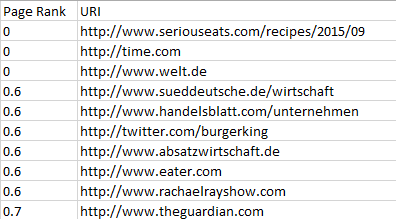
\includegraphics[scale=0.80]{pagerank.png}
        \caption{Page rank along with 10 URIs}
        \label{Page rank along with 10 URIs}
    \end{center}
\end{figure}

\subsubsection{Comparison between Pagerank and TFIDF}
\begin{figure}[ht]    
    \begin{center}
        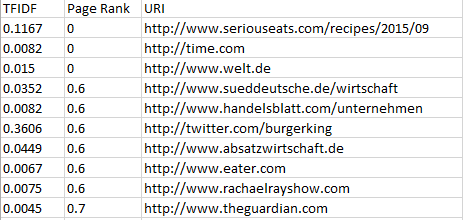
\includegraphics[scale=0.80]{pagerank_tfidf.png}
        \caption{Comparison between Pagerank and TFIDF}
        \label{Comparison between Pagerank and TFIDF}
    \end{center}
\end{figure}
\newpage
